\documentclass[a4paper, 10pt]{article}
\linespread{1.33}
% ┌─────────────────────┐
% │     preamble.tex    │
% └─────────────────────┘

% ══════════ [1] Basic document settings ══════════
\usepackage{fullpage}
\usepackage{geometry}
\geometry{
    top = 2cm,
    bottom = 4.5cm,
    left = 2.5cm,
    right = 2.5cm
}
\usepackage{lastpage}

\usepackage{xcolor}
\usepackage{graphicx}
\usepackage{tikz}
\usepackage{pgfplots}

\usepackage{enumerate}
\usepackage{sectsty}
\subsectionfont{\color{blue}}
\usepackage{enumitem}
\usepackage{array}
\newcolumntype{P}[1]{>{\centering\arraybackslash}p{#1}}

\usepackage{fourier-orns}
\usetikzlibrary{decorations.text}
\pgfplotsset{compat = newest}
\newcommand{\seprule}{
    \vspace*{1.5em}
    \vspace{-8pt}\hrulefill
    \raisebox{-2.1pt}{\quad\decofourleft\decotwo\decofourright\quad}\hrulefill
    \vspace*{1.5em}
}

\usepackage{hyperref}
\hypersetup{
  colorlinks=true,
  linkcolor=blue,
  linkbordercolor={0 0 1},
  urlcolor=blue
}

\usepackage{fancyhdr}
\usepackage[]{mdframed}

\renewcommand{\thesubsection}{\S{} \arabic{section}.\arabic{subsection}}

% ══════════ [2] Math packages ══════════
\usepackage{amsmath}
\usepackage{amsthm}
\usepackage{amsfonts}
\usepackage{amssymb}
\usepackage{amscd}
\usepackage{mathrsfs}
\usepackage{cancel}

% ══════════ [3] Miscellaneous & Fonts ══════════
\setlength{\parindent}{0.0in}
\setlength{\parskip}{0.05in}
\renewcommand{\footrulewidth}{0.4pt}

\usepackage{mathpazo}
\usepackage{domitian}
\usepackage[T1]{fontenc}
\let\oldstylenums\oldstyle
\setmonofont[Scale = 0.8]{DejaVu Sans Mono}

% ══════════ [4] amsthm setup ══════════

\newtheorem{theorem}{Theorem}[section]
\newtheorem{corollary}[theorem]{Corollary}
\newtheorem{lemma}[theorem]{Lemma}

\theoremstyle{definition}
\newtheorem{definition}[theorem]{Definition}

\theoremstyle{remark}
\newtheorem*{remark}{Remark}

\theoremstyle{definition}
\newtheorem{obs}[theorem]{Observation}

\theoremstyle{definition}
\newtheorem{exercise}[theorem]{Exercise}
\newmdtheoremenv[innertopmargin = 8pt,
                 innerbottommargin = 10pt]{exer}[theorem]{Exercise}

\theoremstyle{definition}
\newtheorem{example}[theorem]{Example}
% ┌─────────────────────┐
% │   usercommand.tex   │
% └─────────────────────┘

% ══════════ [1] short-hand notations ══════════
\newcommand{\mbf}{\mathbf}
\newcommand{\mrm}{\mathrm}
\newcommand{\mca}{\mathcal}
\newcommand{\msc}{\mathsc}
\newcommand{\mbb}{\mathbb}
\newcommand{\msf}{\mathsf}

\newcommand{\tbf}{\textbf}
\newcommand{\tit}{\textit}

\newcommand{\eps}{\epsilon}
\newcommand{\kB}{k_{\mathrm{B}}}
\def\dbar{{\mathchar'26\mkern-12mu d}}
\newcommand{\contradiction}{\ensuremath{{\Rightarrow\mspace{-2mu}\Leftarrow}}}
\newcommand{\im}{\mathrm{im}\,}
\renewcommand{\d}{\mathrm{d}}

\renewcommand\qedsymbol{$\blacksquare$}

\newcommand\lecturenumber{07}
\newcommand\lecturedate{Nov 22, 2024}

\pagestyle{fancyplain}
\headheight 40pt
\lhead{Lecture \lecturenumber\\CNBC Deep Learning Subgroup}
\rhead{Riemannian Geometry for Deep Learning \\\lecturedate}
\cfoot{Fall 2024, SNU}
\rfoot{\small\thepage}
\headsep 1.5em

\begin{document}
\setcounter{section}{5}
\section{Lie Derivatives}

\subsection{Flows}

\begin{definition}[Integral curves]
    Let $X$ be a vector field in $\mca{M}$. An \tbf{integral curve} $x(t)$ of $X$ is a curve in $\mca{M}$, whose tangent vector at $x(t)$ is $X|_{x}$.

    \begin{figure}[htbp]
        \centering
        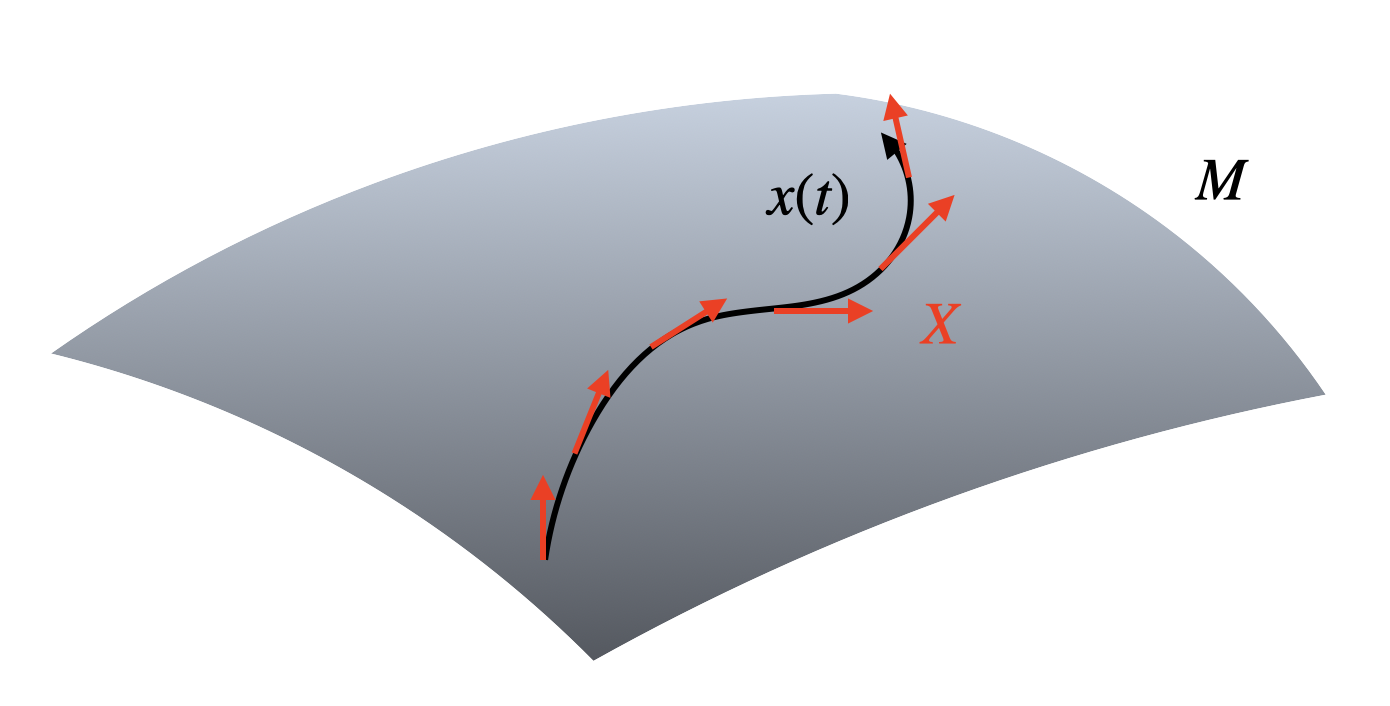
\includegraphics[width=0.5\linewidth]{../images/lecture07/7_01.png}
    \end{figure}

    Given a chart $(U,\varphi)$, this means
    \[ \boxed{\frac{\d{x}^{\mu}(t)}{\d{t}} = X^{\mu}(x(t))} \]
    Here, $x^{\mu}(t)$ denotes the $\mu$-th component of $\varphi\circ x(t)$\footnote{abuse of notation.} and $X^{\mu}$ denotes the $\mu$-th component of $X|_{x}$.
\end{definition}

\begin{remark}
    Finding an integral curve is equivalent to solving the system of ODEs with the initial condition $x_{0}^{\mu} = x^{\mu}(0)$. Hence, unique solution is guaranteed.
\end{remark}

\begin{definition}[Flows]
    Let $\sigma(t, x_{0})$ be an integral curve of $X$, which passes a point $x_{0}$ at $t = 0$. Then $\sigma$ satisfies
    \[ \frac{\d}{\d{t}}\sigma^{\mu}(t,x_{0}) = X^{\mu}(\sigma(t,x_{0})) \;\text{and}\; \sigma^{\mu}(0,x_{0}) = x_{0}^{\mu} \]
    The map $\sigma \,:\, \mbb{R} \times \mca{M} \rightarrow \mca{M}$ is called a \tbf{flow} generated by $X \in \mathscr{X}(\mca{M})$.
\end{definition}

\begin{remark}
    Flows satisfy $\sigma(t, \sigma(s, x)) = \sigma(t + s, x)$ for all $t$ and $s$.
\end{remark}

\begin{definition}
    For fixed $t \in \mbb{R}$, a flow $\sigma(t, x)$ is a \tit{diffeomorphism} from $\mca{M}$ to $\mca{M}$, $\sigma_{t} \,:\, \mca{M} \rightarrow \mca{M}$. $\sigma_{t}$ is made into a \tit{commutative group} by the following rules.
    \begin{itemize}
        \item[(i)] $\sigma_{t} \circ \sigma_{s} = \sigma_{t+s} = \sigma_{s} \circ \sigma_{t}$
        \item[(ii)] $\sigma_{0}$ is the identity map.
        \item[(iii)] $\sigma_{-t} = (\sigma_{t})^{-1}$.
    \end{itemize}
    This group is the \tbf{one-parameter group of transformations}.
\end{definition}

\begin{remark}
    One-parameter group of transformations is \tit{locally} isomorphic to $(\mbb{R}, +)$, but not globally.
\end{remark}
\newpage

% ===== ===== ===== ===== ===== ===== ===== ===== ===== ===== ===== ===== ===== ===== 

\begin{obs}
    With an infinitesimal $\eps$,
    \[ \sigma_{\eps}^{\mu}(x) = \sigma^{\mu}(\eps, x) = x^{\mu} + \eps X^{\mu}(x) \]
    In this context, the vector field $X$ is called the \tbf{infinitesimal generator} of $\sigma_{t}$. The flow $\sigma$ is often referred to as the \tbf{exponentiation} of $X$.
    \begin{align*}
        \sigma^{\mu}(t,x) &= x^{\mu} + t\frac{\d}{\d{s}}\left.\sigma^{\mu}(s,x)\right|_{s=0} + \frac{t^{2}}{2!}\frac{\d^{2}}{\d{s}^{2}}\left|\sigma^{\mu}(s,x)\right|_{s=0} + \cdots \\
        &= \exp\left(t\frac{\d}{\d{s}}\right)\sigma^{\mu}(s,x)|_{s=0} = e^{tX}x^{\mu}_{0}
    \end{align*}
    The flow satisfies the following \tit{exponential properties}.
    \begin{itemize}
        \item[(i)] $\sigma(0, x) = x = \exp(0x)x$
        \item[(ii)] $\displaystyle{\frac{\d\sigma(t,x)}{\d{t}} = X\exp(tX)x}$
        \item[(iii)] $\sigma(t, \sigma(s,x)) = \sigma(t, \exp(sX)x) = e^{tX}e^{sX}x = e^{(t+s)X}x = \sigma(t+s, x)$
    \end{itemize}
\end{obs}

\subsection{Lie Derivatives}

\begin{obs}
    Let $\sigma(t,x)$ and $\tau(t, x)$ be two flows generated by the vector fields $X$ and $Y$.

    \begin{figure}[htbp]
        \centering
        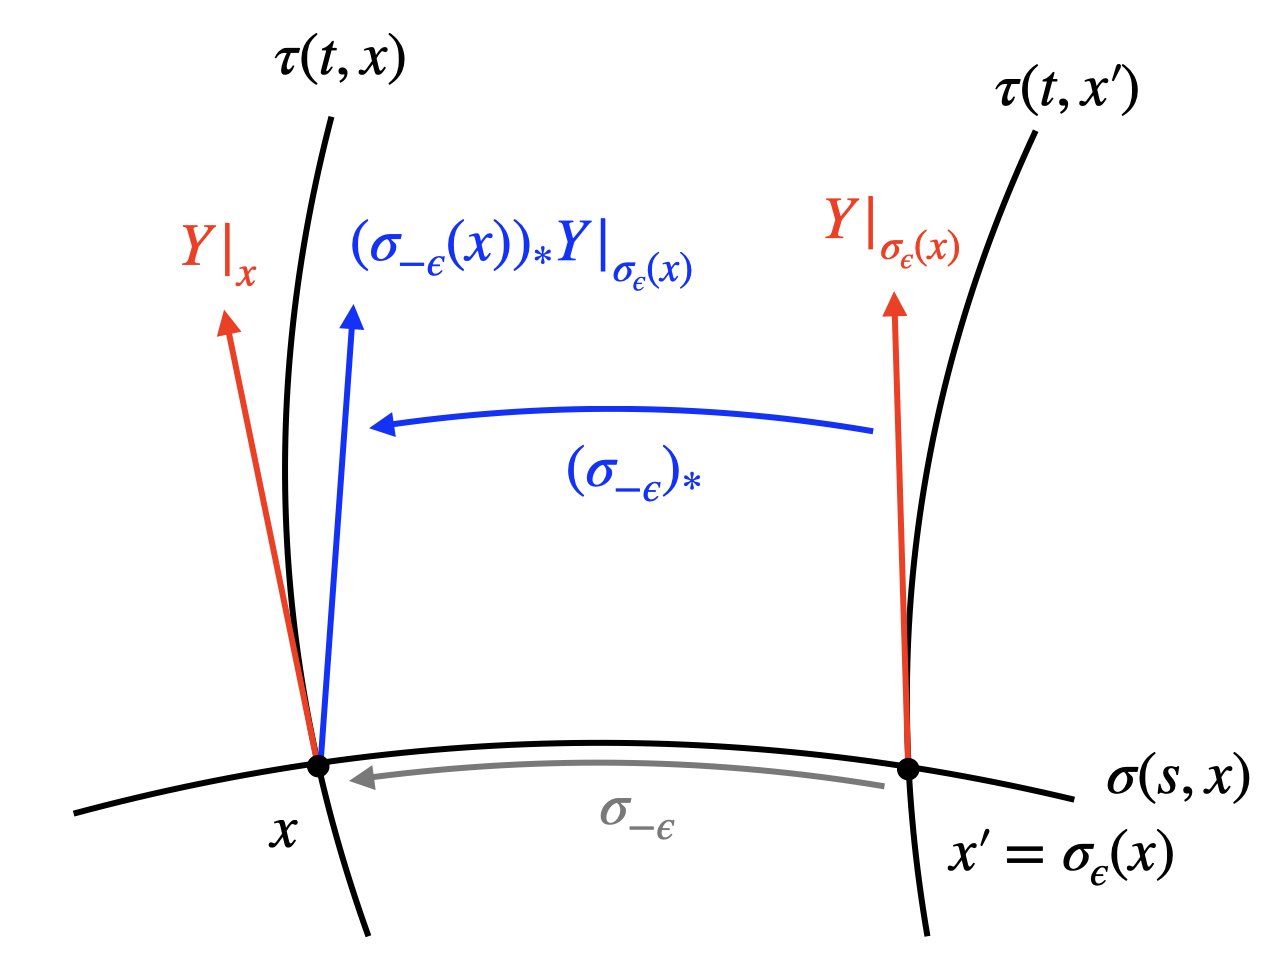
\includegraphics[width=0.5\linewidth]{../images/lecture07/7_02.png}
    \end{figure}
    \[ \frac{\d\sigma^{\mu}(s, x)}{\d{s}} = X^{\mu}(\sigma(s,x)) \;\text{and}\; \frac{\d\tau^{\mu}(t, x)}{\d{t}} = Y^{\mu}(\sigma(t,x)) \]
    Then what is the change of the vector field $Y$ along $\sigma(s, x)$?

    \boxed{Problem.} $Y|_{x}$ (lives in $T_{x}\mca{M}$) and $Y|_{\sigma_{\eps}(x)}$ (lives in $T_{\sigma_{\eps}(x)}\mca{M}$) live in different spaces.

    \boxed{Answer.} To define a sensible derivative, we first map $Y|_{\sigma_{\eps}(x)}$ to $T_{x}\mca{M}$ by \tbf{pushforward map} of $\sigma_{-\eps}$,
    \[ (\sigma_{-\eps})_{\ast} \,:\, T_{\sigma_{\eps}(x)}\mca{M} \rightarrow T_{x}\mca{M} \]
    after which we take a difference between two vectors.
\end{obs}
\newpage

% ===== ===== ===== ===== ===== ===== ===== ===== ===== ===== ===== ===== ===== ===== 

\begin{definition}[Lie derivatives]
    The \tbf{Lie derivative} of a vector field $Y$ along the flow $\sigma$ of $X$ is defined by
    \[ \boxed{\mca{L}_{X}Y \equiv \lim_{\eps \rightarrow 0}\frac{1}{\eps}[(\sigma_{-\eps})_{\ast}Y|_{\sigma_{\eps}(x)} - Y|_{x}]} \]
\end{definition}

\seprule

\begin{obs}
    Let $(U, \varphi)$ be a chart with the coordinates $x^{\mu}$ and
    \[ X = X^{\mu}\frac{\partial}{\partial{x}^{\mu}},\; Y = Y^{\mu}\frac{\partial}{\partial{x}^{\mu}} \]
    be vector fields defined on $U$. Here, we use \tit{coordinate basis}
    \[ \frac{\partial}{\partial{x}^{\mu}} := e_{\mu}|_{x} \]
    where RHS denotes the basis vector at $x$. Then from \tbf{Observation 6.4},
    \[ Y|_{\sigma_{\eps}(x)} = Y^{\mu}(x^{\nu} + \eps X^{\nu}(x)) \cdot e_{\mu}|_{x+\eps X} \simeq [Y^{\mu}(x) + \eps X^{\nu}(x)\partial_{\nu}Y^{\mu}(x)] e_{\mu}|_{x+\eps X} \]
    Now map this vector defined at $\sigma_{\eps}(x)$ to $x$ by $(\sigma_{-\eps})_{\ast} \,:\, T_{\sigma_{\eps}(x)}\mca{M} \rightarrow T_{x}\mca{M}$.
    \begin{align*}
        (\sigma_{-\eps})_{\ast}Y|_{\sigma_{\eps}(x)} &= [Y^{\mu}(x) + \eps X^{\lambda}(x)\partial_{\lambda}Y^{\mu}(x)] \frac{\partial x^{\nu}}{\partial(\sigma_{\eps}(x))^{\mu}} e_{\nu}|_{x} \\
        &= [Y^{\mu}(x) + \eps X^{\lambda}(x)\partial_{\lambda}Y^{\mu}(x)][\delta_{\mu}{}^{\nu}-\eps\partial_{\mu}X^{\nu}]e_{\nu}|_{x} \\
        &= \underbrace{Y^{\mu}(x)e_{\mu}|_{x}}_{Y|_{x}} + \eps[X^{\mu}(x)\partial_{\mu}Y^{\nu}(x) - Y^{\nu}(x)\partial_{\mu}X^{\nu}(x)]e_{\nu}|_{x} + \mca{O}(\eps^{2})
    \end{align*}
    Since
    \[ \frac{\partial x^{\nu}}{\partial(\sigma_{\eps}(x))^{\mu}} = \frac{\partial(\sigma_{-\eps}(x))^{\nu}}{\partial x^{\mu}} = \partial_{\mu}[x^{\nu} - \eps X^{\nu}] = \delta_{\mu}{}^{\nu} - \eps\partial_{\mu}X^{\nu} \]
    In conclusion,
    \[ \boxed{\mca{L}_{X}Y = [X^{\mu}\partial_{\mu}Y^{\nu} - Y^{\mu}\partial_{\mu}X^{\nu}]e_{\nu}} \]
    This is how we differentiate the vector field on the manifolds.
\end{obs}

\begin{definition}[Lie brackets]
    Let $X = X^{\mu}\partial_{\mu}$ and $Y = Y^{\mu}\partial_{\mu}$ be vector fields in $\mca{M}$. The \tbf{Lie bracket} is defined by
    \[ [X,Y]f = X[Y[f]] - Y[X[f]] \quad(f \in \mca{F}(\mca{M}) \]
    Then
    \begin{align*}
        [X,Y]f &= X^{\mu}\partial_{\mu}(Y^{\nu}\partial_{\nu}f) - Y^{\mu}\partial_{\mu}(X^{\nu}\partial_{\nu}f) \\
        &= X^{\mu}(\partial_{\mu}Y^{\nu})(\partial_{\nu}f) + \cancel{X^{\mu}Y^{\nu}\partial_{\mu}\partial_{\nu}f} - Y^{\mu}(\partial_{\mu}X^{\nu})(\partial_{\nu}f) - \cancel{X^{\nu}Y^{\mu}\partial_{\mu}\partial_{\nu}f} \\
        &= (X^{\mu}\partial_{\mu}Y^{\nu} - Y^{\mu}\partial_{\mu}X^{\nu})\partial_{\nu} \cdot f = \mca{L}_{X}Y\cdot f
    \end{align*}
    Hence, Lie derivative is equivalent to Lie bracket.
    \[ \boxed{\mca{L}_{X}Y = [X, Y]} \]
\end{definition}

\end{document}
